% !TEX root = ../thesis_main.tex
\chapter{Prior Ultrafast Spectroscopy Studies of SWCNTs}

\section{The Effect of Dopants on Carrier Dynamics}

\begin{figure}[ht]
	\centering
	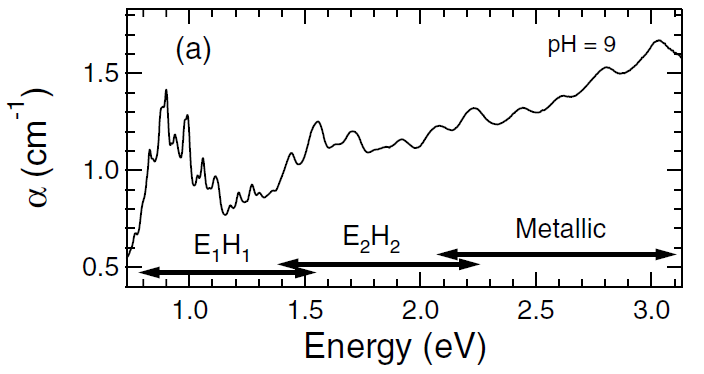
\includegraphics[scale=0.7]{images/chapter_prior_works/abs_gordana}

	\caption{Optical absorption spectrum of dispersed HiPCo SWCNTs. The spectrum contains optical resonances associated with semiconducting nanotubes which include $E_{11}$ in the region denoted as $E_{1} H_{1}$ as well as  $E_{22}$ in the region labeled as $E_{2} H_{2}$. The remaining resonances in the Metallic region come from the $E_{11}$ resonances of metallic nanotubes. Reproduced and modified from Ref.\ \cite{ostojic2004interband}.}

	\label{fig:abs_gordana}
\end{figure}

Ostojic et al.\ (2004) presented an early work regarding the carrier recombination dynamics of carbon nanotubes \cite{ostojic2004interband}. They conducted wavelength-dependent, degenerate pump-probe measurements using an optical parametric amplifier (See Section \ref{section:opa} for details regarding the function of optical parametric amplifiers) whereby the pump and probe have the same photon energy. The sample they studied consisted of a dispersion of HiPCo SWCNTs (See Sections \ref{section:cnt_synthesis} and \ref{section:dispersion_swcnt} for details).

Figure \ref{fig:abs_gordana} shows the optical absorption spectrum of their sample which indicates the presence of many different chiralities, including both metallic and semiconducting nanotubes. The spectral region spanning $E_{1} H_{1}$ contains optical resonances associated with the $E_{11}$ transition occurring in semiconducting nanotubes. The region defined as $E_{2} H_{2}$ contains $E_{22}$ transitions of semiconducting nanotubes. Finally, the region defined as Metallic exhibits the remaining $E_{11}$ resonances emerging from metallic nanotubes.

\begin{figure}[ht]
	\centering
	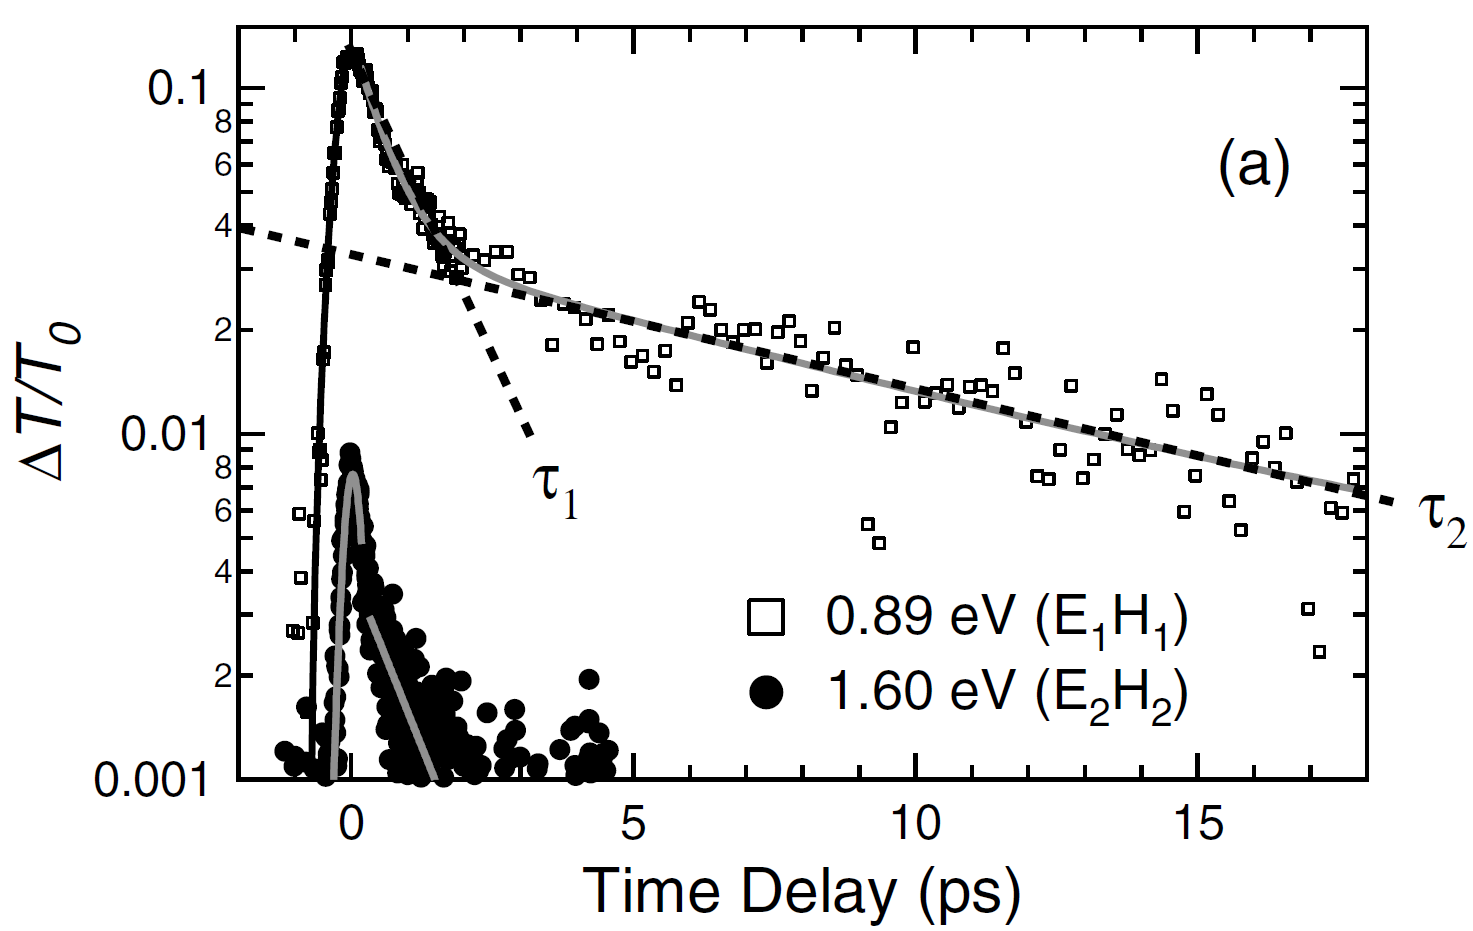
\includegraphics[scale=0.3]{images/chapter_prior_works/dtt_gordana}
	\caption{{\color{red} UNFINISHED } Reproduced and modified from Ref.\ \cite{ostojic2004interband}}
	\label{fig: abs_gordana}
\end{figure}

The observed carrier dynamics showed a clear wavelength dependence as shown in Figure \ref{fig:dtt_ph_gordana}. For pumping and probing within the $E_2 H_2$ region, carrier was best described by a single exponential decay process which was interpreted as intra-band relaxation to lower-energy states. In contrast, a bi-exponential decay process was observed when pumping and probing in the $E_1 H_1$ region. The initial, fast decay was interpreted as intra-band relaxation. Whereas, the following slow exponential decay process was interpreted as inter-band relaxation. At the time of publication, this slow exponential decay process had not been observed before.

Ostojic et al.\  also note that for any chosen wavelength in their degenerate pump-probe study, some nanotubes are resonantly excited whereas others are photo-excited in a non-resonant fashion. This can affect the observed carrier decay dynamics. Figure \ref{fig:wl_dep_gordana} demonstrates this behavior. When photo-exciting the sample at an optical resonance, the ratio between the slow and fast decay times reaches a local maximum. In contrast, when pumping at spectral regions that do not exhibit a well-defined resonance, this ratio diminishes.

\begin{figure}[ht]
	\centering
	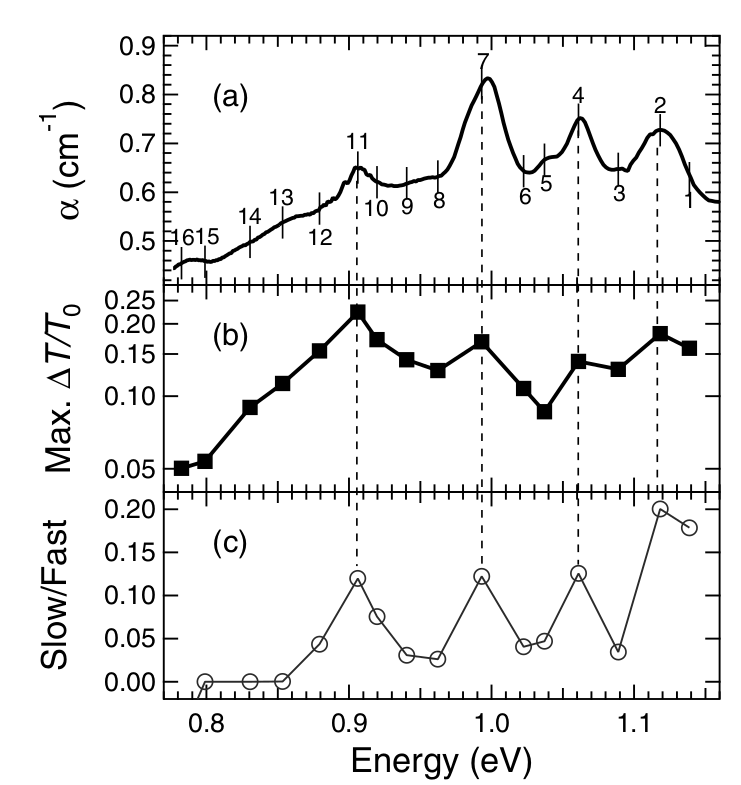
\includegraphics[scale=0.3]{images/chapter_prior_works/wavelength_dependence_gordana}
	\caption{(a) Optical absorption spectrum of the HiPCo SWCNT dispersion. The labeled positions indicate photon energies at which pump-probe measurements were taken. (b) } Reproduced and modified from Ref.\ \cite{ostojic2004interband}}
	\label{fig:wl_dep_gordana}
\end{figure}


Hence, resonant excitation enhances the appearance of interband recombination dynamics. Whereas, non-resonant excitations are more associated with the fast intra-band dynamics. This suggests that the reported decay times only yield statistical averages of the carrier lifetime of the ensemble of all nanotubes that have optical resonances at energies less than or equal to the pump photon energy. Furthermore, they acknowledge that they did not observe a clear correlation between the power of the optical pump and the observed carrier decay times. This excludes the observation of any nonlinear, nonradiative recombination mechanisms such as Auger recombination or exciton-exciton annihilation.


Moreover, decreasing the pH of the sample appeared to mitigate the presence of the slow exponential decay process as shown in Figure \ref{fig:dtt_ph_gordana}. This was interpreted as a consequence of the Burstein-Moss effect. In other words, H+ ions of the acidic aqeuous suspension actively dope suspended SWCNTs. believed that this may cause Fermi level to be somewhere within the conduction band for some population of CNTs such as metallic tubes. Relationship between PL and absorption. At low enough pH, slow decay process goes away along with photoluminescence.

\begin{figure}[ht]
	\centering
	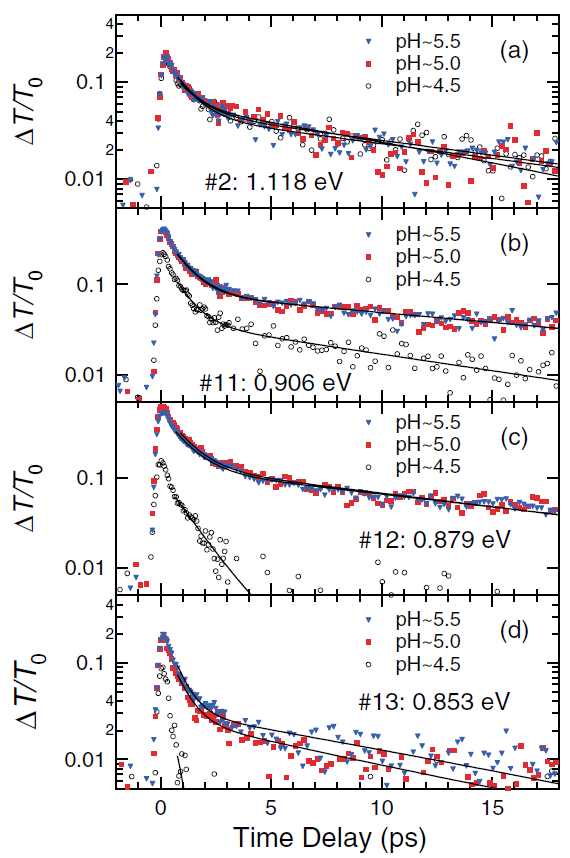
\includegraphics[scale=0.55]{images/chapter_prior_works/dtt_ph_gordana}
	\caption{{\color{red} UNFINISHED } Reproduced and modified from Ref.\ \cite{ostojic2004interband}}
	\label{fig:dtt_ph_gordana}
\end{figure}



\section{Fast Relaxation to E$_\text{11}$ }

\section{The Limits of Exciton-Exciton Annihilation}

Efficient exciton-exciton annihilation \cite{murakami2009existence}.

\begin{figure}[h]
	\centering
	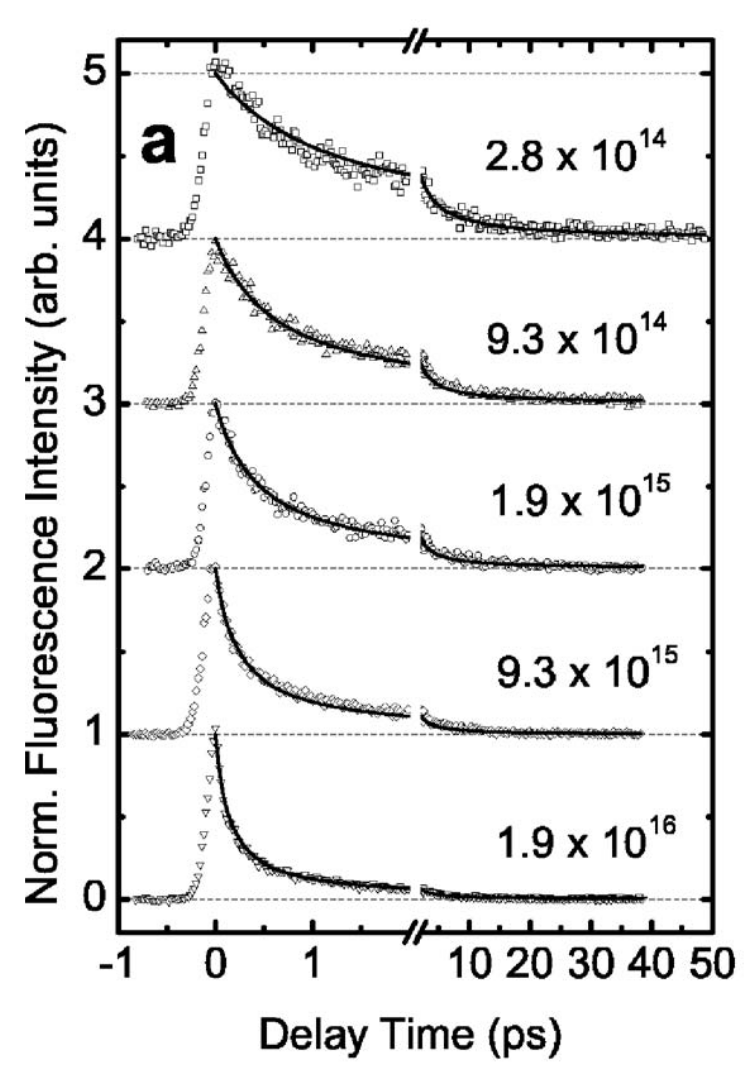
\includegraphics[scale=0.4]{images/chapter_prior_works/pl_valkunas}
	\caption{Reproduced from Ref.\ \cite{valkunas2006exciton}}
\end{figure}

\begin{equation}
\label{eq:exc_annih}
\ce{X + X $\rightarrow$ X},
\end{equation}


\section{Possible Presence of Bi-excitons and Trions}

\begin{figure}[h]
	\centering
	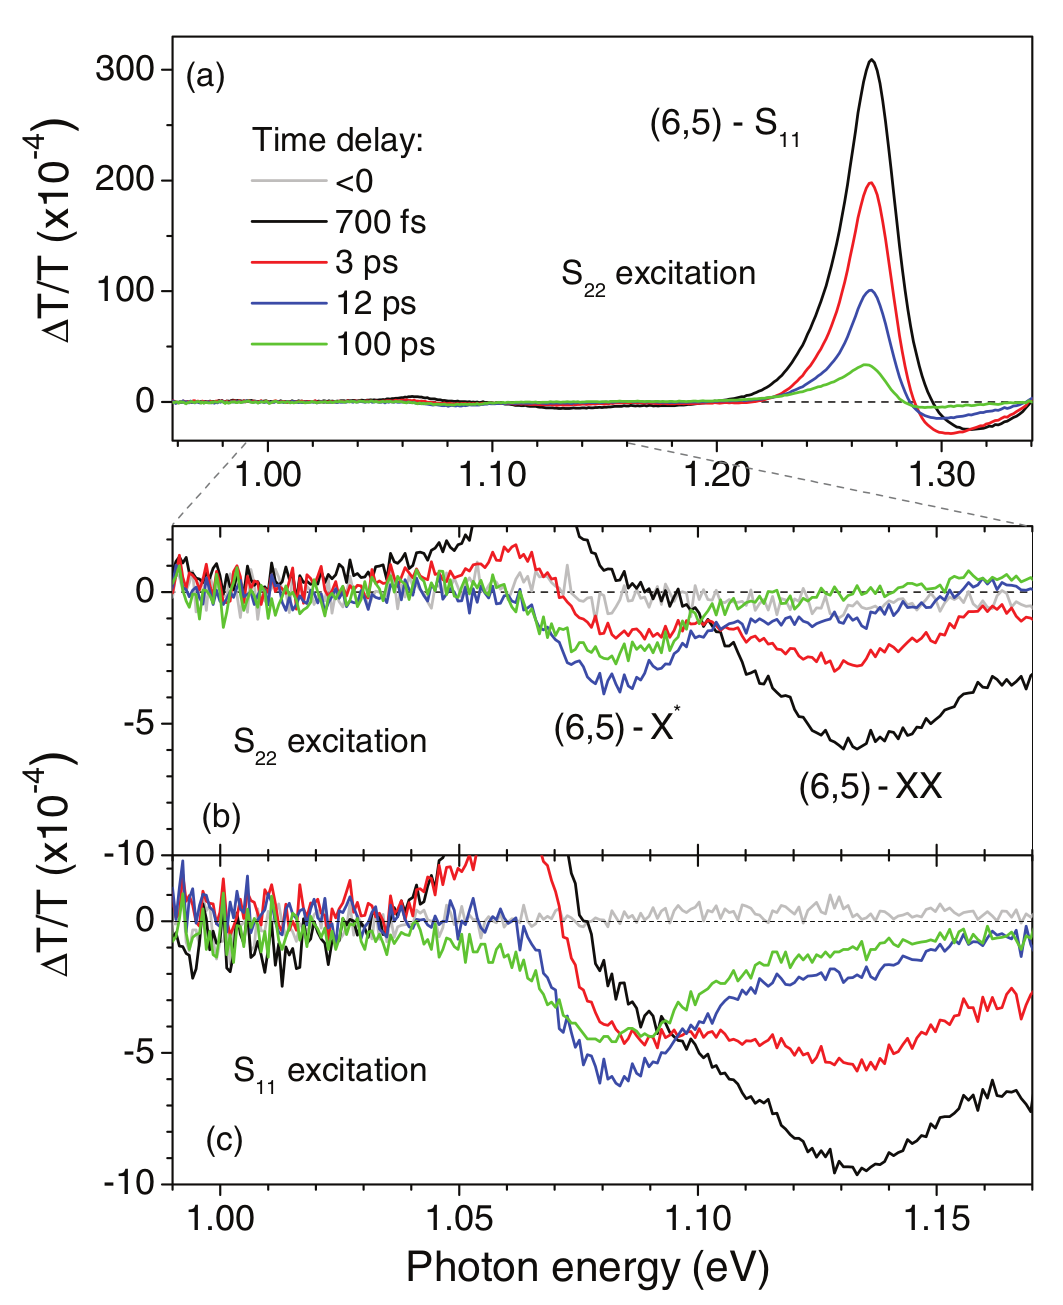
\includegraphics[scale=0.3]{images/chapter_prior_works/dtt_yuma}
	\caption{{\color{red} UNFINISHED} Reproduced from Ref.\ \cite{yuma2013biexciton}.}
\end{figure}

Manzoni et.\ al.\ measured intra-band relaxation rates from $E_{22}$ states to $E_{11}$ states. Used HiPCo CNT film samples.  Found that this occurs over a timescale of 150 fs \cite{manzoni2005intersubband}.

Exciton-Exciton annihilation \cite{valkunas2006exciton, yuma2013biexciton}.
They also show that exciton-exciton annihilation occurs over a time scale such that it is hard to reach Mott densitty of excitons where excitons immediately dissociate to form plasma of free carriers. These a
Apparently, excitons dissociate into free electron-hole pairs before recombination occurs \cite{kumamoto2014spontaneous}.




\section{Summary}
